\documentclass[11pt]{article}
%%% style file you will need for some commands%%%%%%%%%%%%%%%%%%%%%%
%% aahomework is the style file I have used to typeset many commands, feel free to use them in your solutions.
%% bear in mind that if you need to define your command then you will have to make sure that it is not in conflict to my pre-defined command. Otherwise you will need to either use
%% commands defined by me or edit the style file appropriately.
\usepackage{aahomework}
\usepackage{graphicx}
\graphicspath{ {images/} }
\usepackage{tikz}
\usepackage{tipa}
\usepackage{color}
\newcommand*\circled[1]{\tikz[baseline=(char.base)]{
            \node[shape=circle,draw,inner sep=2pt] (char) {#1};}}
%%%the \circled command has been used to create text inside circle for grading table.

\newcommand{\redx}{\textcolor{red}{X}}

%%%\geometry{letterpaper, textwidth=17cm, textheight=22cm}

%%%%%%%%%%%%%%%%%%%%%%%%%%%%%%%%%%%% the following is for the cover sheet--FILL IN appropriately%%
\newcommand{\mycourse}{Introduction to Computer Linguistics 8.1008}
\newcommand{\semesteryear}{Spring 2016}
\newcommand{\myname}{Timothy Fairman, Kaitlin Hipkin, Tyler Wilgenbusch}  %%<<<<<<<<<<<<<<<|========================================= (please put your name here)==========
\newcommand{\hwnumber}{1} %%<<<<<<<<<<<<<<<|========================================= (please put HW number here, e.g. 1,2,3...)==========

%%%%%%%%%%%%%%%%%%%%%%%%%%%%%%%%%%%%%% following is NOT to be edited, DO NOT type anything here, it will receive inputs from what you fill above%%%%%%%%%%%%%%%%%%
\title{Homework \hwnumber} %% DO NOT type in HW number here
\author{\myname} %% DO NOT type in your name here.
\date{\textbf{\mycourse} \hfill {\today} \hfill \textbf{\semesteryear}} %% DO NOT TYPE in mycourse and/or quarteryear values
%%%%%%%%%%%%%%%%%%%%%%%%%%%%%%%%%%%%%%%%%%%%%%%%%%%%%%%%%%%%%%%%%%%%%%%%%%%%%%%%%%%%%%%%%%%%%%%%%%%%%%%%%%%%%%%%%%%%%%%%%%%%%%%%

\setlength{\parindent}{0pt} %% paragraphs will not be indented
\setlength{\parskip}{.25cm} %% space between paragraphs
\linespread{1.1}

\begin{document}
\thispagestyle{empty} %%this is to supress the page number on the cover page

\clearpage %% these are to reset the page number for the first page of your homework to 1.
\pagenumbering{arabic} %% these are to reset the page number for the first page of your homework to 1.
\maketitle

%%%%%%%%%%%%%%%%%%%%%%%%%%%%%%%%% you may start typing below%%%%%%%%%%%%%%%%%%%%%%%%%%%%%%%%%%%%%%%
%% In my style file aahomework.sty I have defined two environments "problem" and "solution" that can be used to type in your question and answer respectively as shown below.%%

\begin{problem}{1}
\textbf{Regular expressions \& FSAs}
\begin{description}
	\item[a.] Write a RE accepting the language that consists of the set comprising all 4 different forms of Peter Bosch's UOS email address: \\
	\textsf{ \{pbosch@uos.de, peter.bosch@uos.de, pbosch@uni‐osnabrueck.de, peter.bosch@uni‐osnabrueck.de\} }
 
	\item[b.] Find an FSA for the language given by the RE /(ab*)+/ . Define this FSA in the format of a formal definition as a 5-tuple, as e.g. on slide 35 of the 2nd lecture.
	\item[c.] Define the same language by means of a regular grammar, as e.g. on slide 37 of lecture 2.
\end{description}
\end{problem}

\newpage

\begin{solution}
\begin{description}
	\item[a.] \begin{verbatim}p(eter\.)?bosch@u(ni-)?os(nabrueck)?\.de\end{verbatim}
	\item[b.] The FSA $F$ for /(ab*)+/ can be defined with the following 5-tuple:\\
	Let $F = <Q, \Sigma, q_{0}, F, \delta(q, i)>$, such that:

	\begin{tabular}{l | l}
		$Q$ & $\{ q_{0}, q_{1}\}$ \\
		$\Sigma$ & $\{a, b\}$ \\
		$q_{0}$ & $q_{0}$ \\
		$F$ & $\{ q_{1} \}$ \\
		$\delta(q, i)$ &  $\{ (q_{0},a,q_{1}), (q_{1}, b, q_{1}), (q_{1}, \varepsilon, q_{0}) \}$
	\end{tabular}

	\begin{figure}[h]
		\centering
		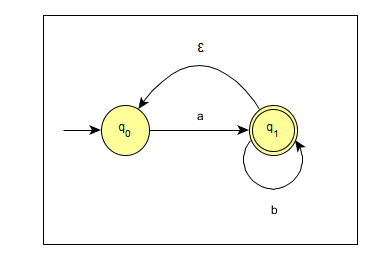
\includegraphics[width=7cm, height=5cm]{fsa} \\
		\caption{FSA for /(ab*)+/}
	\end{figure}
	\item[c.] The regular grammer $G$ for /(ab*)+/ can be defined with the following 4-tuple: \\
	Let $G = <N, \Sigma, S, P>$ such that:

	\begin{tabular}{l | l}
		$N$ & $\{ S, A\}$ \\
		$\Sigma$ & $\{a, b\}$ \\
		$S$ & $S$ \\
		$P$ & 
		\begin{tabular}{| l c l |} \hline 
			$S$ & $\rightarrow$ & $aA$ \\ 
			$A$ & $\rightarrow$ & $bA$ \\ 
			$A$ & $\rightarrow$ & $S$  \\
			$A$ & $\rightarrow$ & $\varepsilon$ \\
			\hline
		\end{tabular}
	\end{tabular}

\end{description}

\end{solution}

\vspace*{0.5cm} %% this is to put some vertical space betwen the next problem and the previous solution. You can change the value to something more appropriate.
\newpage

\begin{problem}{2}
\textbf{English consonants} \\
If your native language is not English, or you are uncertain as to your pronounciation, you are advised to
consult the phonetic transcriptions in a dictionary. In any case of doubt, the intended pronunciation is RP
(i.e., "BBC English"). 

\begin{description}
	\item[a.] The words in the left-hand column below \textit{begin} with 22 different consonants. The words in the right-hand columns begin with the same 22 consonants, but in a different order. Match each word on the left with the word on the right which has the same initial consonant (sound, not letter), and write down the solutions as pairs of letters and numbers, e.g."k2".

	\begin{tabular}{l p{6cm} | r l}
		a & tomato & 1 & bag \\
		b & Czech & 2 & cat \\
		c & yacht & 3 & cent \\
		d & loose & 4 & check \\
		e & there & 5 & dude \\
		f & guess & 6 & fan \\
		g & chef & 7 & gas \\
		h & dare & 8 & gem \\
		i & vote & 9 & leap \\
		j & kneel & 10 & meek \\
		k & kite & 11 & nail \\
		l & holy & 12 & pain \\
		m & pest & 13 & ptomaine \\
		n & phone & 14 & room \\
		o & jest & 15 & shave \\
		p & zest & 16 & then \\
		q & send & 17 & thick \\
		r & rhyme & 18 & vest \\
		s & main & 19 & weight \\
		t & thin & 20 & whole \\
		u & boom & 21 & young \\
		v & wild & 22 & zoom 
	\end{tabular}
	\newpage
	\item[b.] The words in the left-hand columns below \textit{end} with 21 different consonants. The words in the right-hand columns have the same final consonants, but in a different order. Match each word on the left with the word on the right which has the same final consonant and write down the solutions as pairs of letters and numbers, e.g. "c4".
	
	\begin{tabular}{l p{6cm} | r l}
		a & love & 1 & both \\
		b & rogue & 2 & car \\
		c & dome & 3 & clothe \\
		d & grub & 4 & dumb \\
		e & smooth & 5 & fate \\
		f & ridge & 6 & globe \\
		g & sane & 7 & graph \\
		h & beige & 8 & lace \\
		i & lung & 9 & look \\
		j & gruff & 10 & odd \\
		k & eight & 11 & phrase \\
		l & fade & 12 & pole \\
		m & toll & 13 & rage \\
		n & daze & 14 & rich \\
		o & lock & 15 & rouge \\
		p & loss & 16 & rug \\
		q & hope & 17 & save \\
		r & youth & 18 & sign \\
		s & care & 19 & soap \\
		t & ash & 20 & tongue \\
		u & witch & 21 & wash
	\end{tabular}

	\newpage
	\item[c.] This time match the \textit{final} consonant of each word in the left-hand columns with the \textit{initial} consonant of a word in the right-hand columns - \textbf{if there is such a match}. Write down the solutions as pairs of letters and numbers, e.g., "a3". If there is no match write "x -".

	\begin{tabular}{l p{6cm} | r l}
		a & pitch &   1 & beige \\
		b & team & 2 & breathe \\  
		c & kill & 3 & chip \\  
		d & bad & 4 & coach \\  
		e & dame & 5 & comb \\  
		f & goal & 6 & cough \\  
		g & choke & 7 & door \\  
		h & jell & 8 & face \\  
		i & fun & 9 & lane \\  
		j & think & 10 & ledge \\  
		k & safe & 11 & lick \\  
		l & vain & 12 & maid \\  
		m & they & 13 & meat \\  
		n & zone & 14 & nave \\  
		o & mode & 15 & nose \\  
		p & name & 16 & robe \\  
		q & lace & 17 & rogue \\  
		r & rake & 18 & rung \\  
		s & yell & 19 & rush \\  
		t & wet & 20 & Ruth \\  
		u & head & 21 & sail \\  
		v & shift &  & 
	\end{tabular}

\end{description}

\end{problem}

\newpage

\begin{solution}
The correct pairings are as follows:

\begin{description}
	\item[a.] Pairings of initial consonants:

	\begin{tabular}{l l | l}
	\textbf{Pairs} & \textbf{Words} & \textbf{English Phoneme} \\ \hline
	a, 13 & tomato, ptomaine & /\textipa{t}/ \\
	b, 4 & Czech, check & /\textipa{tS}/ \\
	c, 21 & yacht, young & /\textipa{j}/ \\
	d, 9 & loose, leap & /\textipa{l}/ \\
	e, 16 & there, then & /\textipa{D}/ \\
	f, 7 & guess, gas & /\textipa{g}/ \\
	g, 15 & chef, shave & /\textipa{S}/ \\
	h, 5 & dare, dude & /\textipa{d}/ \\
	i, 18 & vote, vest & /\textipa{v}/ \\
	j, 11 & kneel, nail & /\textipa{n}/ \\
	k, 2 & kite, cat & /\textipa{k}/ \\
	l, 20 & holy, whole & /\textipa{h}/ \\
	m, 12 & pest, pain & /\textipa{p}/ \\
	n, 6 & phone, fan & /\textipa{f}/ \\
	o, 8 & jest, gem & /\textipa{dZ}/ \\
	p, 22 & zest, zoom & /\textipa{z}/ \\
	q, 3 & send, cent & /\textipa{s}/ \\
	r, 14 & rhyme, room & /\textipa{r}/ \\
	s, 10 & main, meek & /\textipa{m}/ \\
	t, 17 & thin, thick & /\textipa{T}/ \\
	u, 1 & boom, bag & /\textipa{b}/ \\
	v, 19 & wild, weight & /\textipa{w}/ \\
	\hline
	\end{tabular}
	
	\newpage

	\item[b.] Pairings of end consonants: 

	\begin{tabular}{l l | l}
	\textbf{Pairs} & \textbf{Words} & \textbf{English Phoneme} \\ \hline
	a, 17 & love, save & /\textipa{v}/ \\
	b, 16 & rogue, rug & /\textipa{g}/ \\
	c, 4 & dome, dumb & /\textipa{m}/ \\
	d, 6 & grub, globe & /\textipa{b}/ \\
	e, 3 & smooth, clothe & /\textipa{D}/ \\
	f, 13 & ridge, rage & /\textipa{dZ}/ \\
	g, 18 & sane, sign & /\textipa{n}/ \\
	h, 15 & beige, rouge & /\textipa{Z}/ \\
	i, 20 & lung, tongue & /\textipa{N}/ \\
	j, 7 & gruff, graph & /\textipa{f}/ \\
	k, 5 & eight, fate & /\textipa{t}/ \\
	l, 10 & fade, odd & /\textipa{d}/ \\
	m, 12 & toll, pole & /\textipa{l}/ \\
	n, 11 & daze, phrase & /\textipa{z}/ \\
	o, 9 & lock, look & /\textipa{k}/ \\
	p, 8 & loss, lace & /\textipa{s}/ \\
	q, 19 & hope, soap & /\textipa{p}/ \\
	r, 1 & youth, both & /\textipa{T}/ \\
	s, 2 & care, car & /\textipa{r}/ \\
	t, 21 & ash, wash & /\textipa{S}/ \\
	u, 14 & witch, rich & /\textipa{tS}/ \\
	\hline
	\end{tabular}

	\newpage

	\item[c.] Pairings of \textbf{final} consonants of the words in the \textbf{left-hand} column with \textbf{initial} consonants of the words in the \textbf{right-hand} column:

	\begin{tabular}{l l | l}
	\textbf{Pairs} & \textbf{Words} & \textbf{English Phoneme} \\ \hline
	a, 3 & pitch, chip & /\textipa{tS}/ \\
	b, 12 & team, maid & /\textipa{m}/ \\
	e, 13 & dame, meat & /\textipa{m}/ \\
	p, 13 & name, meat & /\textipa{m}/ \\
	c, 9 & kill, lane & /\textipa{l}/ \\
	f, 10 & goal, ledge & /\textipa{l}/ \\
	h, 11 & jell, lick & /\textipa{l}/ \\
	s, 11 & yell, lick & /\textipa{l}/ \\
	d, 7 & bad, door & /\textipa{d}/ \\
	o, 7 & mode, door & /\textipa{d}/ \\
	u, 7 & head, door & /\textipa{d}/ \\
	g, 4 & choke, coach & /\textipa{k}/ \\
	j, 5 & think, comb & /\textipa{k}/ \\
	r, 6 & rake, cough & /\textipa{k}/ \\
	i, 14 & fun, nave & /\textipa{n}/ \\
	l, 15 & vain, nose & /\textipa{n}/ \\
	n, 15 & zone, nose & /\textipa{n}/ \\
	k, 8 & safe, face & /\textipa{f}/ \\
	m, \redx & they, \redx & /\textipa{D}/ \\
	q, 21 & lace, sail & /\textipa{s}/ \\
	t, \redx & wet, \redx & /\textipa{t}/ \\
	v, \redx & shift, \redx & /\textipa{t}/ \\
	\hline
	\end{tabular} \\

	Note that some words from right-hand column can be matched to more than one word in the left-hand column (i.e. [dame, meat] and [name, meat]).  Below are all the unmatched, right-hand column words:

	\begin{tabular}{l l | l}	
	\textbf{Pairs} & \textbf{Words} & \textbf{English Phoneme} \\ \hline
	\redx, 1 & \redx, beige & /\textipa{b}/ \\
	\redx, 2 & \redx, breathe & /\textipa{b}/ \\
	\redx, 16 & \redx, robe & /\textipa{r}/ \\
	\redx, 17 & \redx, rogue & /\textipa{r}/ \\
	\redx, 18 & \redx, rung & /\textipa{r}/ \\
	\redx, 19 & \redx, rush & /\textipa{r}/ \\
	\redx, 20 & \redx, Ruth & /\textipa{r}/ \\
	\hline
	\end{tabular}

\end{description}

\end{solution}

\end{document}